\clearpage
\section{\RU{Множество Мандельброта}\EN{Mandelbrot set}}
\label{Mandelbrot_demo}

\RU{Я нашел дему}\EN{I have found a demo}\footnote{\EN{Download it}\RU{Можно скачать} \href{http://go.yurichev.com/17306}
{\RU{здесь}\EN{here}},} 
\RU{написанную автором по имени}\EN{written by} ``Sir\_Lagsalot'' \InENRU 2009, 
\RU{рисующая множество Мандельброта, и это программа для x86 с размером файла всего 64 байта}\EN{that draws 
the Mandelbrot set, which is just a x86 program with executable 
file size of only 64 bytes}.
\RU{Там только 30 16-битных x86-инструкций}\EN{There are only 30 16-bit x86 instructions}.

\RU{Вот что она рисует}\EN{Here it is what it draws}:

\begin{figure}[H]
\centering
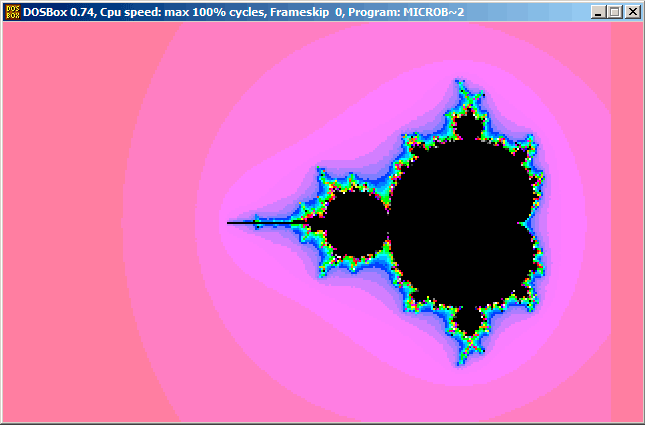
\includegraphics[scale=\FigScale]{examples/demos/mandelbrot/1.png}
\end{figure}

\RU{Попробуем разобраться, как она работает}\EN{Let's try to understand how it works}.

\clearpage
\subsection{\RU{Теория}\EN{Theory}}

\subsubsection{\RU{Немного о комплексных числах}\EN{A word about complex numbers}}

\RU{Комплексное число состоит из двух чисел (вещественная (Re) и мнимая (Im).}
\EN{A complex number is a number that consists of two parts --- real (Re) and imaginary (Im).}

\RU{Комплексная плоскость --- это двухмерная плоскость, где любое комплексное число может быть расположено:
вещественная часть --- это одна координата и мнимая --- вторая.}
\EN{The complex plane is a two-dimensional plane where any complex number can be placed: the real part is one coordinate
and the imaginary part is the other.}

\RU{Некоторые базовые правила, которые нам понадобятся}\EN{Some basic rules we need to know}:

\begin{itemize}
\item \RU{Сложение}\EN{Addition}: $(a+bi) + (c+di) = (a+c) + (b+d)i$

\RU{Другими словами}\EN{In other words}:

$\operatorname{Re}(sum) = \operatorname{Re}(a) + \operatorname{Re}(b)$

$\operatorname{Im}(sum) = \operatorname{Im}(a) + \operatorname{Im}(b)$

\item \RU{Умножение}\EN{Multiplication}: $(a+bi) (c+di) = (ac-bd) + (bc+ad)i$

\RU{Другими словами}\EN{In other words}:

$\operatorname{Re}(product) = \operatorname{Re}(a) \cdot \operatorname{Re}(c) - \operatorname{Re}(b) \cdot \operatorname{Re}(d)$

$\operatorname{Im}(product) = \operatorname{Im}(b) \cdot \operatorname{Im}(c) + \operatorname{Im}(a) \cdot \operatorname{Im}(d)$

\item \RU{Возведение в квадрат}\EN{Square}: $(a+bi)^2 = (a+bi) (a+bi) = (a^2-b^2) + (2ab)i$

\RU{Другими словами}\EN{In other words}:

$\operatorname{Re}(square) = \operatorname{Re}(a)^2-\operatorname{Im}(a)^2$

$\operatorname{Im}(square) = 2 \cdot \operatorname{Re}(a) \cdot \operatorname{Im}(a)$

\end{itemize}

\subsubsection{\RU{Как нарисовать множество Мандельброта}\EN{How to draw the Mandelbrot set}}

\RU{Множество Мандельброта --- это набор точек, для которых рекурсивное соотношение}
\EN{The Mandelbrot set is a set of points for which the} $z_{n+1} = {z_n}^2 + c$ \EN{recursive sequence}
(\RU{где}\EN{where} $z$ \AndENRU $c$ \RU{это комплексные числа и}\EN{are complex numbers and} $c$ 
\RU{это начальное значение}\EN{is the starting value})
\RU{не стремится к бесконечности}\EN{does not approach infinity}.\\
\\
\RU{Простым русским языком}\EN{In plain English language}: 

\begin{itemize}
\item \RU{Перечисляем все точки на экране}\EN{Enumerate all points on screen}. 
\item \RU{Проверяем, является ли эта точка в множестве Мандельброта}\EN{Check if the specific point 
is in the Mandelbrot set}.
\item \RU{Вот как проверить}\EN{Here is how to check it}:

  \begin{itemize}
  \item \RU{Представим точку как комплексное число}\EN{Represent the point as a complex number}.
  \item \RU{Возведем в квадрат}\EN{Calculate the square of it}.
  \item \RU{Прибавим значение точки в самом начале}\EN{Add the starting value of the point to it}.
  \item \RU{Вышло за пределы}\EN{Does it go off limits}? \RU{Прерываемся, если да}\EN{If yes, break}.
  \item \RU{Передвигаем точку в новое место, координаты которого только что вычислили}\EN{Move the point to the 
new place at the coordinates we just calculated}.
  \item \RU{Повторять всё это некое разумное количество итераций}\EN{Repeat all this for some reasonable 
number of iterations}.
  \end{itemize}

\item \RU{Двигающаяся точка в итоге не вышла за пределы}\EN{The point is still in limits}?
\RU{Тогда рисуем точку}\EN{Then draw the point}.

\item \RU{Двигающаяся точка в итоге вышла за пределы}\EN{The point has eventually gone off limits}?

  \begin{itemize}
    \item \RU{(Для черно-белого изображения) ничего не рисуем}\EN{(For a black-white image) do not draw anything}.
    \item 
\RU{(Для цветного изображения) преобразуем количество итераций в какой-нибудь цвет.
Так что цвет будет показывать, с какой скоростью точка вышла за пределы.}
\EN{(For a colored image) transform the number of iterations to some color. 
      So the color shows the speed with which point has gone off limits.}
  \end{itemize}

\end{itemize}

\RU{Я написал алгоритмы для комплексных и обычных целочисленных чисел (на языке, отдаленно напоминающем Python):}
\EN{Here is Pythonesque algorithm I wrote for both complex and integer number representations:}

\lstinputlisting[caption=\RU{Для комплексных чисел}\EN{For complex numbers}]{examples/demos/mandelbrot/algo_cplx.lst.\LANG}

\RU{Целочисленная версия, это версия где все операции над комплексными числами заменены на операции 
с целочисленными, в соответствии с изложенными раннее правилами.}
\EN{The integer version is where the operations on complex numbers are replaced with integer operations according to the rules
I explained above.}

\lstinputlisting[caption=\RU{Для целочисленных чисел}\EN{For integer numbers}]{examples/demos/mandelbrot/algo_int.lst.\LANG}

\RU{Вот также исходный текст на C\#, который я взял из статьи в Wikipedia}\EN{Here is also a C\# source 
I got from the Wikipedia article}\footnote{\href{http://go.yurichev.com/17307}{wikipedia}}, \RU{но я немного изменил его,
чтобы он выдавал количество итераций, вместо некоторого символа}\EN{but I modified it
so it prints the iteration numbers instead of some symbol}
\footnote{\RU{Здесь также и исполняемый файл}\EN{Here is also the executable file}: 
\href{http://go.yurichev.com/17163}{beginners.re}}:

\lstinputlisting{examples/demos/mandelbrot/dump_iterations.cs}

\RU{Вот файл с результатом, который слишком широкий, чтобы привести его здесь}\EN{Here is the resulting file, 
which is too wide to be included here}: \\
\href{http://go.yurichev.com/17164}{beginners.re}.

\RU{Максимальное число итераций 40, так что если вы видите 40 в этом файле, это означает что точка ходила
40 итераций, но так и не вышла за пределы.}
\EN{The maximal number of iterations is 40, so when you see 40 in this dump, it mean that this point was wandering
for 40 iterations but never got off limits.} 
\RU{Номер $n$ меньше 40 означает что эта точка оставалась внутри пределов только $n$ итераций, и затем
вышла наружу.}
\EN{A number $n$ less then 40 mean that point remained inside the bounds only for $n$ iterations, 
then it went outside them.}

\clearpage
\RU{Вот здесь есть неплохая демонстрация:}\EN{There is a cool demo available at} 
\url{http://go.yurichev.com/17309}, \RU{она показывает визуально,
как определенная точка двигается по плоскости на каждой итерации}\EN{which shows
visually how the point moves on the plane at each iteration for some specific point}. 
\RU{Я сделал два скриншота}\EN{I made two screenshots}.

\RU{В начале я кликнул внутри желтой области, и увидел траекторию (зеленые линии), которая в итоге
загручивается в какой-то точке внутри:}
\EN{First, I clicked inside the yellow area and saw that the trajectory (green line) 
eventually swirls at some point inside:}

\begin{figure}[H]
\centering
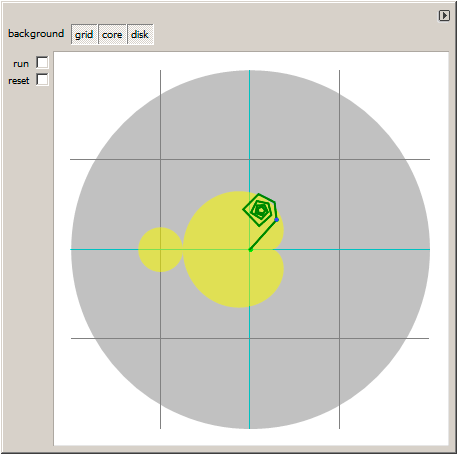
\includegraphics[scale=\FigScale]{examples/demos/mandelbrot/demo1.png}
\caption{\RU{Я кликнул внутри желтой области}\EN{I clicked inside yellow area}}
\end{figure}

\RU{Это значит, что точка на которой я кликнул, находится внутри множества Мандельброта.}
\EN{This implies that the point I clicked belongs to the Mandelbrot set.}

\clearpage
\RU{Затем я кликнул снаружи желтой области, и мы видим более хаотичные движения точки, которая быстро выходит
за пределы:}
\EN{Then I clicked outside the yellow area and saw a much more chaotic point movement, 
which quickly went off bounds:}

\begin{figure}[H]
\centering
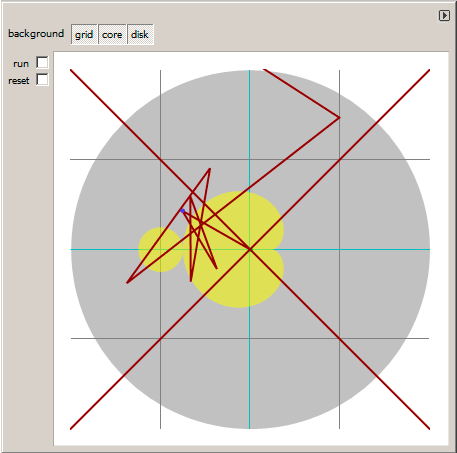
\includegraphics[scale=\FigScale]{examples/demos/mandelbrot/demo2.png}
\caption{\RU{Я кликнул снаружи желтой области}\EN{I clicked outside yellow area}}
\end{figure}

\RU{Это значит, что эта точка не принадлежит множеству Мандельброта}\EN{This mean the point not belongs 
to Mandelbrot set}.

\RU{Другая неплохая демонстрация там}\EN{Another good demo is available here}: 
\url{http://go.yurichev.com/17310}.

\clearpage
\subsection{\RU{Вернемся к демо}\EN{Let's get back to the demo}}

\RU{Демо, хотя и крошечная (только 64 байта или 30 инструкций), реализует общий алгоритм, изложенный
здесь, но с некоторыми трюками.}
\EN{The demo, although very tiny (just 64 bytes or 30 instructions), implements the common algorithm 
I described here, but using some coding tricks.}

\RU{Исходный код можно скачать, так что вот он, но я также добавил своих комментариев}\EN{The source code is 
easily downloadable, so I got it, but I also added my comments}:

\lstinputlisting[caption=\RU{Исходный код с комментариями}\EN{Commented source code},numbers=left]{examples/demos/mandelbrot/Microbrot_commented.asm.\LANG}

\RU{Алгоритм}\EN{Algorithm}:

\begin{itemize}
\item \RU{Переключаемся в режим VGA}\EN{Switch to} 320*200 \RU{256 цветов}\EN{VGA video mode, 256 colors}. 
$320*200=64000$ (0xFA00). 
\RU{Каждый пиксель кодируется одним байтом, так что размер буфера 0xFA00 байт.}
\EN{Each pixel is encoded by one byte, so the buffer size is 0xFA00 bytes.}
\RU{Он адресуется здесь при помощи пары регистров ES:DI}\EN{It is addressed using the ES:DI registers pair}.

\index{x86!\Registers!ES}
ES \RU{должен быть здесь}\EN{must be} 0xA000\RU{, потому что это сегментный адрес видеобуфера, но запись
числа 0xA000 в ES потрубет по крайней мере 4 байта}\EN{ here, because this is the segment address of 
the VGA video buffer, but storing 0xA000 to ES requires at least 4 bytes} (\TT{PUSH 0A000h / POP ES}). 
\RU{О 16-битной модели памяти в MS-DOS, читайте больше тут}\EN{You can read more about the 16-bit MS-DOS memory model here}: 
\myref{8086_memory_model}.

\index{x86!\Instructions!LES}
\RU{Учитывая, что BX здесь 0, и Program Segment Prefix находится по нулевому адресу, 2-байтная инструкция
\TT{LES AX,[BX]} запишет 0x20CD в AX и 0x9FFF в ES.}
\EN{Assuming that BX is zero here, and the Program Segment Prefix is at the zeroth
address, the 2-byte \TT{LES AX,[BX]} instruction stores 0x20CD to AX and 0x9FFF to ES.}
\RU{Так что программа начнет рисовать на 16 пикселей (или байт) перед видеобуфером.}
\EN{So the program starts to draw 16 pixels (or bytes) before the actual video buffer.}
\RU{Но это}\EN{But this is} MS-DOS, 
\RU{здесь нет защиты памяти, так что ничего плохого не произойдет.}
\EN{there is no memory protection, so no crash can happen.}
\RU{Вот почему вы видите красную полосу шириной 16 пикселей справа}\EN{That's why you see a red strip 16 
pixels wide at the right side}.
\RU{Вся картинка сдвинута налево на 16 пикселей}\EN{The whole picture is shifted left by 16 pixels}.
\RU{Это цена экономии 2-х байт}\EN{This is the price of saving 2 bytes}.

\item \RU{Вечный цикл, обрабатывающий каждый пиксель}\EN{A infinite loop processes each pixel}.
\RU{Наверное, самый общий метод обойти все точки на экране это два цикла:
один для X-координаты, второй для Y-координаты.}
\EN{Probably, the most common way to enumerate all pixels on the screen is with two loops: 
one for the X coordinate, another for the Y coordinate.}
\RU{Но тогда вам придется перемножать координаты для поиска байта в видеобуфере VGA}\EN{But then you'll need 
to multiply the coordinates to address a byte in the VGA video buffer}.
\RU{Автор этого демо решил сделать наоборот: перебирать все байты в видеобуфере при помощи одного цикла
вместо двух и затем получать координаты текущей точки при помощи деления.}
\EN{The author of this demo decided to do it otherwise: enumerate all bytes in the video buffer by using one single loop instead 
of two, and get the coordinates of the current point using division.}
\RU{В итоге координаты такие: X в пределах}\EN{The resulting coordinates are: X in the range of} $-100..99$ \AndENRU Y 
\RU{в пределах}\EN{in the range of} $-256..63$.
\RU{Вы можете увидеть на скриншоте что картинка как бы сдвинута в правую часть экрана}\EN{You can see on 
the screenshot that the picture is somewhat shifted to the right part of screen}.
\RU{Это потому что самая большая черная дыра в форме сердца обычно появляется на координатах 0,0 и они
здесь сдвинуты вправо.}
\EN{That's because the biggest heart-shaped black hole usually appears on coordinates 0,0 and these are shifted
here to right.}
\RU{Мог ли автор просто отнять 160 от X, чтобы получилось значение в пределах}\EN{Could the author just 
subtract 160 from the value to get X in the range of} $-160..159$? 
\RU{Да, но инструкция}\EN{Yes, but the instruction} \TT{SUB DX, 160} \RU{занимает 4 байта}\EN{takes 4 bytes}, 
\RU{тогда как}\EN{while} \TT{DEC DH}\EMDASH{}2 \RU{байта}\EN{bytes} 
(\RU{которая отнимает}\EN{which subtracts} 0x100 (256) \RU{от}\EN{from} DX). 
\RU{Так что картинка сдвинута ценой экономии еще 2-х байт}\EN{So the whole picture is shifted for the cost of 
another 2 bytes of saved space}.

    \begin{itemize}
    \item \RU{Проверить, является ли текущая точка внутри множества Мандельброта}\EN{Check, if the current 
point is inside the Mandelbrot set}.
          \RU{Алгоритм такой же, как я описал}\EN{The algorithm is the one that I described}.
\index{x86!\Instructions!LOOP}
     \item \RU{Цикл организуется инструкцией \TT{LOOP}, которая использует регистр CX как счетчик}\EN{The loop 
is organized using the \TT{LOOP} instruction, which uses the CX register as counter}.
\RU{Автор мог бы установить число итераций на какое-то число, но не сделал этого: потому что 320 уже
находится в CX (было установлено на строке 35), и это итак подходящее число как число максимальных
итераций.}
\EN{The author could set the number of iterations to some specific number, but he didn't: 320 is already present in CX 
(was set at line 35), and this is good maximal iteration number anyway.}
\RU{Мы здесь экономим немного места, не загружая другое значение в регистр CX}\EN{We save here some space 
by not the reloading CX register with another value}.

\index{x86!\Instructions!SAR}
     \item \RU{Здесь используется \TT{IMUL} вместо \TT{MUL}, потому что мы работаем с знаковыми значениями:
помните, что координаты 0,0 должны быть где-то рядом с центром экрана.}
\EN{\TT{IMUL} is used here instead of \TT{MUL}, because we work with signed values: 
remember that the 0,0 coordinates has to be somewhere near the center of the screen.}
\RU{Тоже самое и с \TT{SAR} (арифметический сдвиг для знаковых значений): она используется вместо \TT{SHR}.}
\EN{It's the same with \TT{SAR} (arithmetic shift for signed values): it's used instead of \TT{SHR}.}

     \item \RU{Еще одна идея --- это упростить проверку пределов}\EN{Another idea is to simplify the bounds check}.
\RU{Нам бы пришлось проверять пару координат, т.е. две переменных}\EN{We need to check a coordinate pair, 
i.e., two variables}.
\RU{Что делает автор это трижды проверяет на переполнение: две операции возведения в квадрат и одно 
прибавление}\EN{What the author does is to checks thrice for overflow: two squaring operations and one addition}.
\RU{Действительно, мы ведь используем 16-битные регистры, содержащие знаковые значения в пределах}
\EN{Indeed, we use 16-bit registers, which hold signed values in the range of} $-32768..32767$, \RU{так что
если любая из координат больше чем 32767 в процессе умножения, точка однозначно вышла за пределы,
и мы переходим на метку \TT{MandelBreak}.}
\EN{so if any of the coordinates is greater than 32767 during the signed multiplication, this point is definitely out 
of bounds: we jump to the \TT{MandelBreak} label.}

     \item \RU{Здесь также имеется деление на 64 (при помощи инструкции SAR). 64 задает масштаб.}
\EN{There is also a division by 64 (SAR instruction). 64 sets scale.}
\RU{Попробуйте увеличить значение и вы получите более увеличенную картинку, или уменьшить для
меньшей.}
\EN{Try to increase the value and you can get a closer look, or to decrease if for a more distant look.}

    \end{itemize}

\item \RU{Мы находимся на метке}\EN{We are at the} \TT{MandelBreak}\EN{ label}, \RU{есть только две возможности
попасть сюда}\EN{there are two ways of getting here}: 
\RU{цикл закончился с}\EN{the loop ended with} CX=0 (\RU{точка внутри множества Мандельброта}
\EN{the point is inside the Mandelbrot set}); \RU{или потому что произошло переполнение (CX все еще содержит 
какое-то значение)}\EN{or because an overflow has happened (CX still holds some value)}.
\RU{Записываем 8-битную часть CX (CL) в видеобуфер}\EN{Now we write the low 8-bit part of CX (CL) to the 
video buffer}.
\RU{Палитра по умолчанию грубая, тем не менее, 0 это черный: поэтому видим черные дыры в местах где точки
внутри множества Мандельброта.}
\EN{The default palette is rough, nevertheless, 0 is black: hence we see black holes in the places where the points are
in the Mandelbrot set.}
\RU{Палитру можно инициализировать в начале программы, но не забывайте, это всего лишь программа на 64 
байта}\EN{The palette can be initialized at th program's start, but remember, this is only a 64 bytes program}!

\item \RU{Программа работает в вечном цикле, потому что дополнительная проверка, где остановится, 
или пользовательский интерфейс, это дополнительные инструкции}\EN{The program runs in an infinite loop, 
because an additional check where to stop, or any user interface will result in additional instructions}.

\end{itemize}

\RU{Еще оптимизационные трюки}\EN{Some other optimization tricks}:

\begin{itemize}
\index{x86!\Instructions!CWD}
\item \EN{The }1-\RU{байтная}\EN{byte} CWD \RU{используется здесь для обнуления DX вместо двухбайтной}\EN{is used here 
for clearing DX instead of the 2-byte} \TT{XOR DX, DX} \RU{или даже трехбайтной}\EN{or even the 3-byte} \TT{MOV DX, 0}.

\item \EN{The }1-\RU{байтная}\EN{byte} \TT{XCHG AX, CX} \RU{используется вместо двухбайтной}\EN{is used instead of the 2-byte} 
\TT{MOV AX,CX}. 
\RU{Текущее значение в AX все равно уже не нужно}\EN{The current value of AX is not needed here anyway}.

\item DI (\RU{позиция в видеобуфере}\EN{position in video buffer}) \RU{не инициализирована, и будет 0xFFFE в
начале}\EN{is not initialized, and it is 0xFFFE at the start}
\footnote{\RU{Больше о состояниях регистров на старте}\EN{More information about initial register values}: 
\url{http://go.yurichev.com/17004}}.
\RU{Это нормально, потому что программа работает бесконечно для всех DI в пределах 0..0xFFFF, и пользователь
не может увидеть, что работала началась за экраном (последний пиксель видеобуфера 320*200 имеет адрес 0xF9FF).}
\EN{That's OK, because the program works for all DI in the range of 0..0xFFFF eternally, 
and the user can't notice
that it is started off the screen (the last pixel of a 320*200 video buffer is at address 0xF9FF).}
\RU{Так что некоторая часть работы на самом деле происходит за экраном}\EN{So some work is actually done 
off the limits of the screen}.
\RU{А иначе понадобятся дополнительные инструкции для установки DI в 0; добавить проверку на конец буфера.}
\EN{Otherwise, you'll need an additional instructions to set DI to 0 and check for the video buffer's end.}

\end{itemize}

\newcommand{\MyFixedVersion}{\RU{Моя ``исправленная'' версия}\EN{My ``fixed'' version}}
\subsection{\MyFixedVersion}

\lstinputlisting[caption=\MyFixedVersion,numbers=left]{examples/demos/mandelbrot/my_version.asm.\LANG}

\RU{Я попытался исправить все эти странности: теперь палитра плавная черно-белая, видеобуфер на правильном месте
(строки 19..20), картинка рисуется в центре экрана (строка 30), программа в итоге заканчивается и ждет,
пока пользователь нажмет какую-нибудь клавишу (строки 58..68).}
\EN{I made an attempt to fix all these oddities: now the palette is smooth grayscale, the video buffer is at the correct place 
(lines 19..20),
the picture is drawn on center of the screen (line 30), the program eventually ends and waits for the user's keypress 
(lines 58..68).}
\RU{Но теперь она намного больше: 105 байт (или 54 инструкции)}
\EN{But now it's much bigger: 105 bytes (or 54 instructions)}
\footnote{\RU{Можете поэкспериментировать и сами: скачайте DosBox и NASM и компилируйте так:}
\EN{You can experiment by yourself: get DosBox and NASM and compile it as:} 
\TT{nasm fiole.asm -fbin -o file.com}}.

\begin{figure}[H]
\centering
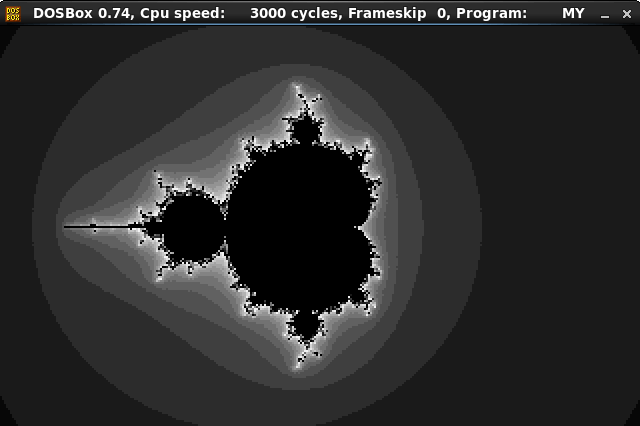
\includegraphics[scale=\FigScale]{examples/demos/mandelbrot/fixed.png}
\caption{\MyFixedVersion}
\label{fig:mandelbrot_fixed}
\end{figure}
